\section{Bausteinsicht}
\label{sec:bausteinsicht}

Die Bausteinsicht zeigt die statische Zerlegung des Systems in
seine Bausteine (Services, Komponenten, Klassen) sowie deren
Abhängigkeiten. Sie beantwortet die Frage: \emph{Aus welchen
Teilen besteht EduPlanner und wie hängen diese zusammen?}

Die Darstellung folgt dem \textbf{Zoom-in-Prinzip} des
arc42-Templates: Ebene~1 zeigt das Gesamtsystem als Whitebox
mit seinen fünf Services und der Infrastruktur. Die Ebenen~2
und~3 zoomen schrittweise in einzelne Bounded Contexts hinein
-- bis hin zu kritischen Klassen und Algorithmen.

Für die Diagramme wird die \textbf{C4-Notation}\footnotemark{}
verwendet. Jede Ebene enthält zunächst ein Diagramm zur
Orientierung, gefolgt von einer Tabelle bzw.\ Auflistung mit
den Verantwortlichkeiten der dargestellten Bausteine.

\footnotetext{%
  \textbf{C4-Modell} (nach Simon Brown). Ein hierarchisches
  Diagrammmodell für Softwarearchitektur mit vier
  Abstraktionsebenen: \emph{Context} (System im Umfeld),
  \emph{Container} (deploybare Einheiten), \emph{Component}
  (logische Bausteine innerhalb eines Containers) und
  \emph{Code} (Klassen/Interfaces). Jede Ebene zoomt tiefer
  in das System hinein.
  Vgl.\ \url{https://c4model.com}.%
}

% ══════════════════════════════════════════════
\subsection{Ebene~1 -- Gesamtsystem (Whitebox)}
\label{sec:baustein-ebene1}

Das folgende C4-Container-Diagramm (Abb.~\ref{fig:container})
zeigt alle deployierbaren Einheiten von EduPlanner sowie die
Kommunikationswege zwischen ihnen. Die fünf fachlichen Services
(blau) entsprechen den Bounded Contexts aus Kapitel~4.
Infrastrukturbausteine (grau) -- API Gateway, Message Broker
und Datenbanken -- sind unterstützende Komponenten ohne eigene
Fachlogik. Externe Systeme (orange) liegen ausserhalb der
Systemgrenze.

\begin{figure}[H]
  \centering
  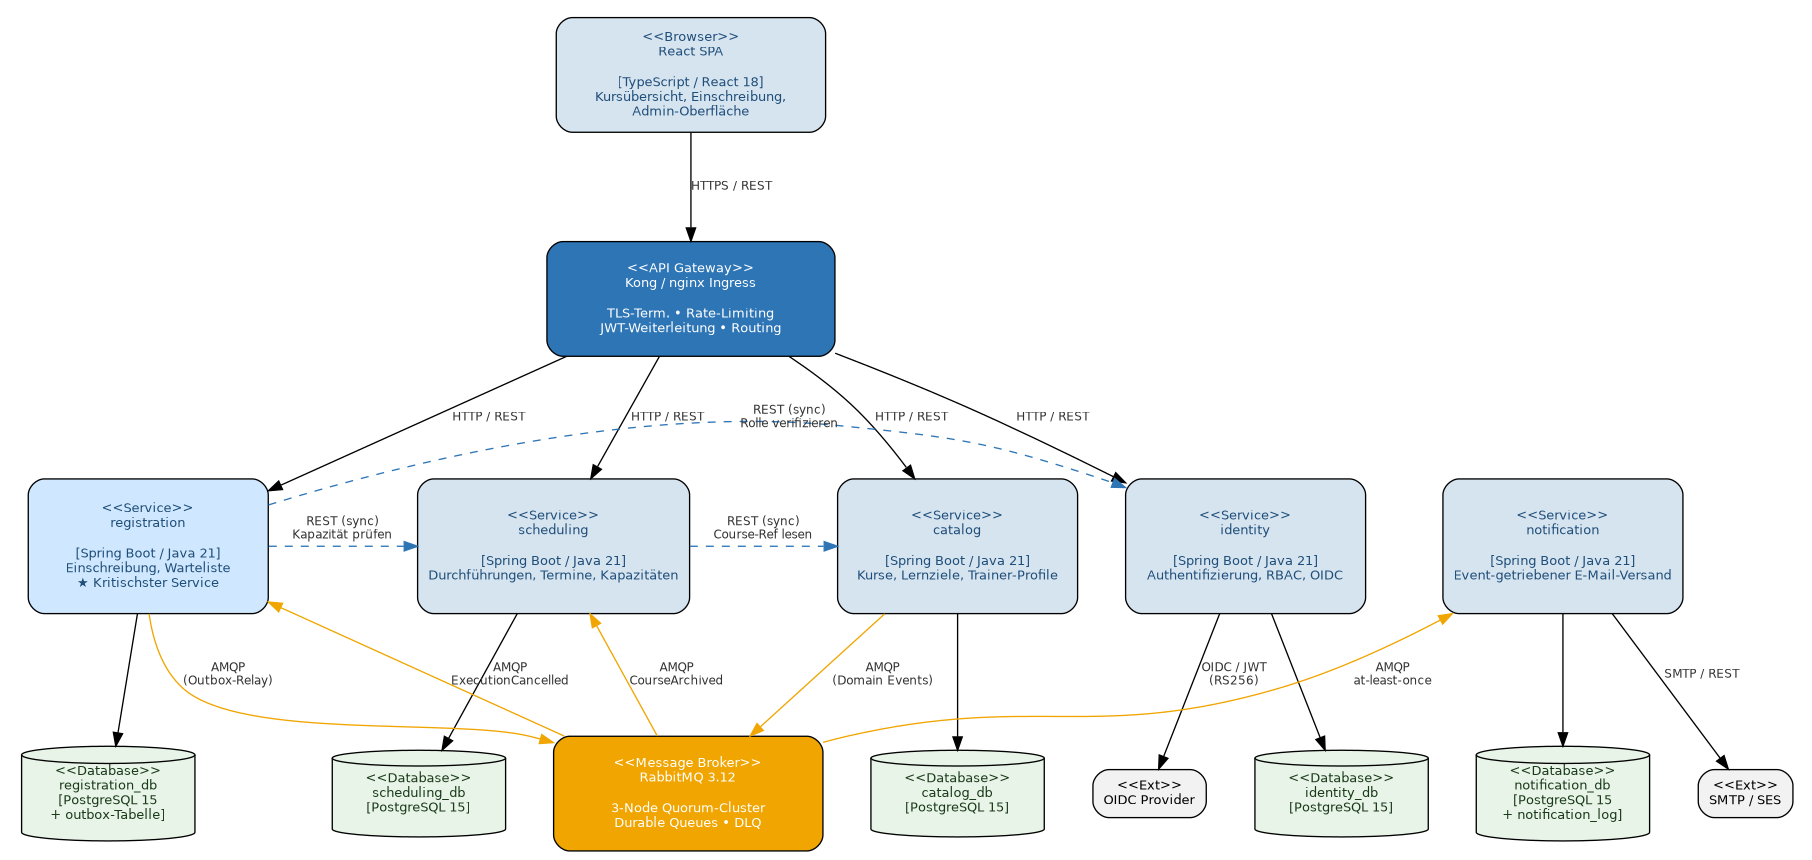
\includegraphics[width=\textwidth]{assets/ebene1_container_diagram}
  \caption{\textit{Ebene~1 -- C4-Container-Diagramm: Gesamtsystem
  EduPlanner mit Services, Infrastruktur und externen
  Systemen.}}
  \label{fig:container}
\end{figure}

Die nachfolgende Tabelle beschreibt die Verantwortlichkeit
jedes Bausteins im Detail:

\begin{tabularx}{\textwidth}{L{2.8cm} X}
  \rowcolor{tableheader}
  \color{white}\textbf{Baustein} &
  \color{white}\textbf{Verantwortlichkeit} \\

  \texttt{catalog} &
  Kursbeschreibungen, Lernziele, Trainer-Profile.
  Publiziert \texttt{CourseCreated},
  \texttt{CoursePublished},
  \texttt{CourseArchived}. \\

  \rowcolor{tablegrey}
  \texttt{scheduling} &
  Planung von Kursdurchführungen inkl.\ Termine,
  Kapazitäten, Trainer-Zuweisung. \\

  \texttt{registration} &
  Einschreibungsverwaltung: Kapazitätsprüfung,
  Warteliste, Stornierungen.
  \textbf{Kritischster Service.} \\

  \rowcolor{tablegrey}
  \texttt{notification} &
  Event-getriebener E-Mail-Versand; kein Einfluss
  auf Kernprozesse. \\

  \texttt{identity} &
  Authentifizierung via OIDC-IdP; Rollen- und
  Benutzerverwaltung. \\

  \rowcolor{tablegrey}
  API Gateway &
  TLS-Terminierung, Rate-Limiting (100~Req/s),
  JWT-Weiterleitung, Routing. \\

  Message Broker &
  Entkoppelte asynchrone Kommunikation via
  Durable Queues und Dead-Letter-Exchange. \\

  \rowcolor{tablegrey}
  Reporting (BFF) &
  v1.0: Dashboard-Daten aus \texttt{catalog} und
  \texttt{registration} separat abgefragt und im
  Frontend aggregiert (BFF-Light via Angular /
  Vue.js). v2.0: Dedizierter Reporting-Service
  geplant (Kap.~14.3). \\
\end{tabularx}

% ══════════════════════════════════════════════
\subsection{Ebene~2 -- Bounded Context: \texttt{catalog}}
\label{sec:baustein-catalog}

Der \texttt{catalog}-Service ist fachlich der einfachste
Bounded Context: Er verwaltet Kursbeschreibungen und
Trainer-Profile und steuert über eine Zustandsmaschine, welche
Kurse für Teilnehmer sichtbar sind. Abbildung~\ref{fig:catalog}
zeigt die internen Bausteine und deren Zusammenspiel -- vom
REST-Controller über die Fachlogik bis hin zur Datenbank und
Event-Publikation.

\begin{figure}[H]
  \centering
  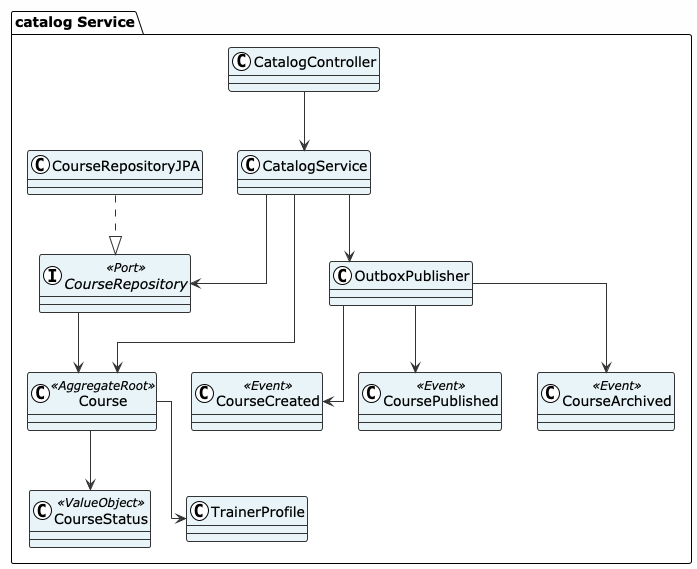
\includegraphics[width=\textwidth]{assets/ebene2_catalog_class_diagram}
  \caption{\textit{Ebene~2 -- UML-Klassendiagramm: Interne
  Bausteine des \texttt{catalog}-Service.}}
  \label{fig:catalog}
\end{figure}

Wichtige Klassen / Aggregate:
\begin{itemize}[leftmargin=1.5em]
  \item \textbf{Course} (Aggregate Root): \texttt{CourseId},
  Titel, Beschreibung, Lernziele,
  \texttt{CourseStatus}
  (Draft $\to$ Published $\to$ Archived), Trainer.
  \item \textbf{TrainerProfile}: Stammdaten, Fachgebiete,
  Verfügbarkeitsstatus.
  \item \textbf{CourseStatus}: Value Object; steuert erlaubte
  Zustandsübergänge (State Machine).
  \item \textbf{CourseRepository}: Port-Interface;
  Implementierung via JPA/Hibernate.
\end{itemize}

\noindent\textbf{Domain Events:}
\begin{itemize}[leftmargin=1.5em, label=\raisebox{0.25ex}{\tiny\(\bullet\)}]
  \item \texttt{CourseCreated} -- Neuer Kurs wurde angelegt
  \item \texttt{CoursePublished} -- Kurs wurde veröffentlicht
  \item \texttt{CourseArchived} -- Kurs wurde archiviert
\end{itemize}

% ──────────────────────────────────────────────
\subsubsection{CourseStatus -- Zustandsübergangsdiagramm}

Das \texttt{CourseStatus}-Value-Object steuert den Lebenszyklus
eines Kurses über eine einfache Zustandsmaschine mit drei
Zuständen und erlaubten Übergängen
(Abb.~\ref{fig:course-state}). Rückwärtsübergänge sind bewusst
nicht vorgesehen (ADR-006): Ein archivierter Kurs kann nicht
reaktiviert werden -- stattdessen muss ein neuer Kurs angelegt
werden.

\begin{figure}[H]
  \centering
  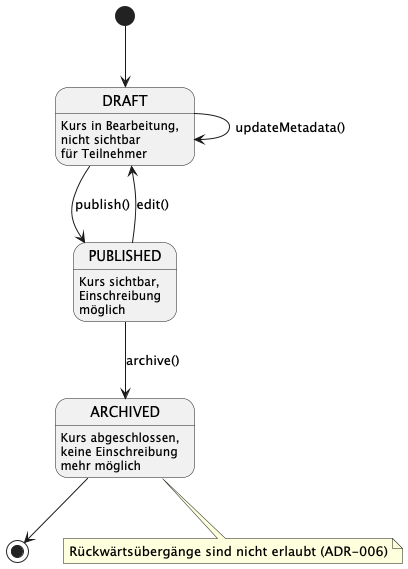
\includegraphics[width=0.55\textwidth]{assets/catalog_course_state_machine}
  \caption{\textit{Zustandsübergangsdiagramm: \texttt{CourseStatus}
  mit den drei Zuständen DRAFT, PUBLISHED und
  ARCHIVED. Rückwärtsübergänge sind nicht vorgesehen.}}
  \label{fig:course-state}
\end{figure}

% ══════════════════════════════════════════════
\subsection{Ebene~2 -- Bounded Context: \texttt{scheduling}}
\label{sec:baustein-scheduling}

Der \texttt{scheduling}-Service ist für die zeitliche und
organisatorische Planung von Kursdurchführungen verantwortlich.
Er referenziert Kurse aus \texttt{catalog} ausschliesslich über
die \texttt{CourseId} (Anti-Corruption Layer) und enthält die
kritische Logik zur Vermeidung von Trainer-Doppelbuchungen.
Abbildung~\ref{fig:scheduling} zeigt seine internen
Komponenten -- man beachte insbesondere den ACL-Baustein rechts,
der die Entkopplung vom \texttt{catalog}-Domänenmodell
sicherstellt.

\begin{figure}[H]
  \centering
  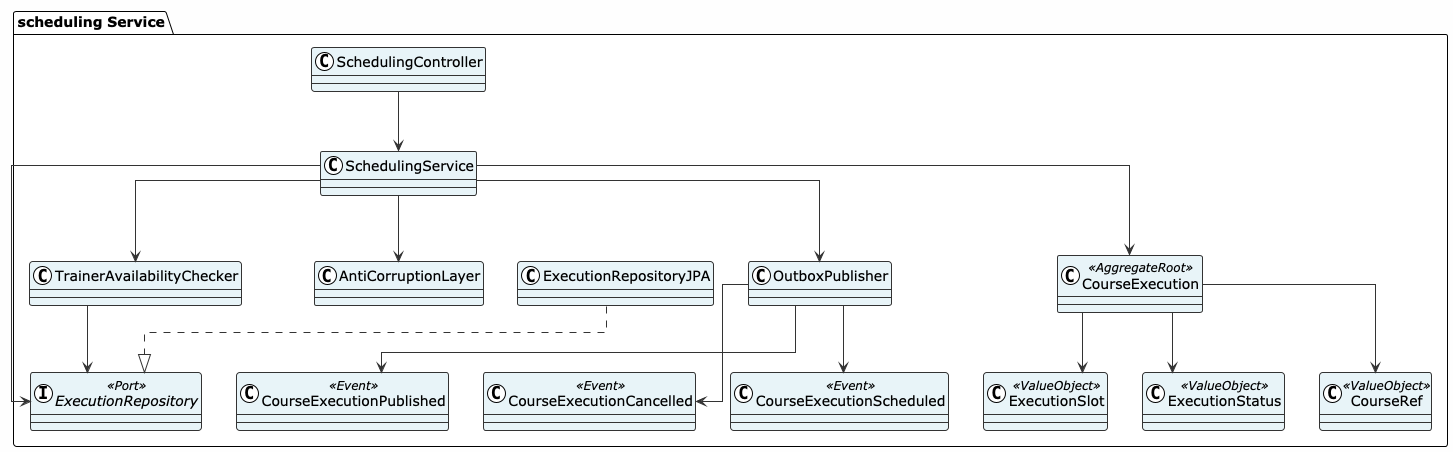
\includegraphics[width=\textwidth]{assets/ebene2_scheduling_class_diagram}
  \caption{\textit{Ebene~2 -- UML-Klassendiagramm: Interne
  Bausteine des \texttt{scheduling}-Service inkl.\
    Anti-Corruption Layer zum \texttt{catalog}-Context.}}
  \label{fig:scheduling}
\end{figure}

Wichtige Klassen / Aggregate:
\begin{itemize}[leftmargin=1.5em]
  \item \textbf{CourseExecution} (Aggregate Root):
  \texttt{CourseRef} (nur ID -- Anti-Corruption Layer),
  Startdatum, Enddatum, Ort, Kapazität,
  \texttt{ExecutionStatus}, Trainer.
  \item \textbf{SchedulingService}: Prüft
  Trainer-Verfügbarkeit und verhindert Überschneidungen.
  Die Prüflogik verwendet transaktionale Locks
  (SELECT\ldots FOR UPDATE) zur Race-Condition-Prävention
  (Details siehe Laufzeitsicht, Kap.~6).
  \item \textbf{ExecutionSlot}: Value Object für einen
  Zeitblock einer Durchführung.
\end{itemize}

\noindent\textbf{Domain Events:}
\begin{itemize}[leftmargin=1.5em, label=\raisebox{0.25ex}{\tiny\(\bullet\)}]
  \item \texttt{CourseExecutionScheduled} -- Durchführung wurde geplant
  \item \texttt{CourseExecutionPublished} -- Durchführung wurde veröffentlicht
  \item \texttt{CourseExecutionCancelled} -- Durchführung wurde abgesagt
\end{itemize}

\paragraph{Fallback-Verhalten bei Ausfall des \texttt{catalog}-Service}

Der \texttt{scheduling}-Service ist abhängig vom
\texttt{catalog}-Service, um Kursnamen zu laden. Sollte
\texttt{catalog} ausfallen oder nicht erreichbar sein, darf dies
die Kernfunktionalität von \texttt{scheduling} nicht blockieren.
Daher implementiert \texttt{scheduling} ein intelligentes
Fallback-Verhalten:

\begin{itemize}[leftmargin=1.5em]
  \item \textbf{Normale Situation}: \texttt{scheduling} ruft
  \texttt{catalog} auf und erhält den Kursnamen
  (z.\,B.\ ``Java Grundlagen'').
  \item \textbf{Ausfall von \texttt{catalog}}: Der
  \texttt{scheduling}-Service erkennt den Fehler über
  einen \textbf{Circuit Breaker} (Resilience4j). Statt
  die Anfrage zu blockieren oder zu fehlschlagen, gibt
  \texttt{scheduling} die Durchführungsdaten mit einem
  Platzhalter zurück: \texttt{[Kursinformation nicht
  verfügbar]}. Die eigentlichen Daten (Termin, Ort,
  Trainer) bleiben korrekt.
  \item \textbf{Circuit Breaker Logik}: Nach 5~Fehlern
  innerhalb von 10~Sekunden geht der Circuit Breaker in
  den Zustand ``OPEN''. Weitere Anfragen an
  \texttt{catalog} werden sofort abgelehnt, ohne zu
  warten. Nach 30~Sekunden wechselt der Circuit Breaker
  in den Zustand ``HALF-OPEN'' und versucht einen
  Testaufruf. Ist dieser erfolgreich, geht der Circuit
  Breaker zurück in den Zustand ``CLOSED''.
\end{itemize}

\textbf{Resultat:} Benutzer sehen zwar, dass Kursinformationen
temporär nicht verfügbar sind, können aber weiterhin auf
Durchführungstermine zugreifen. Dies ist ein Beispiel für
\emph{Graceful Degradation}: Das System funktioniert mit
reduzierter Funktionalität weiter, statt komplett auszufallen.

% ══════════════════════════════════════════════
\subsection{Ebene~2 -- Bounded Context: \texttt{registration}}
\label{sec:baustein-registration}

Der \texttt{registration}-Service ist der \textbf{kritischste
Bounded Context} des Systems: Er verarbeitet Einschreibungen,
verwaltet Wartelisten und muss unter allen Umständen verhindern,
dass mehr Teilnehmer eingeschrieben werden als Plätze vorhanden
sind -- auch bei hoher gleichzeitiger Last. Aus diesem Grund
ist er der einzige Service, für den eine Ebene-3-Sicht
dokumentiert wird
(siehe Abschnitt~\ref{sec:baustein-reg-ebene3}).

Abbildung~\ref{fig:registration} zeigt die internen Komponenten
inkl.\ der beiden kritischen Bausteine
\texttt{CapacityChecker} (Race-Condition-Schutz) und
\texttt{OutboxPublisher} (garantierte Event-Publikation).

\begin{figure}[H]
  \centering
  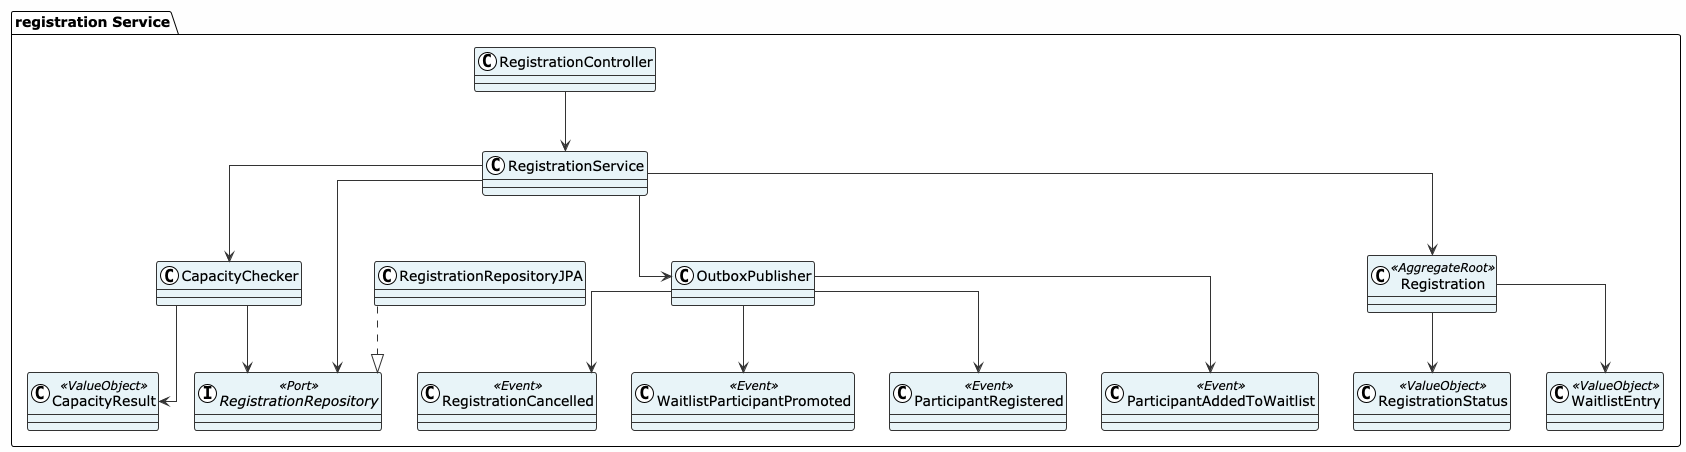
\includegraphics[width=\textwidth]{assets/ebene2_registration_class_diagram}
  \caption{\textit{Ebene~2 -- UML-Klassendiagramm: Interne
  Bausteine des \texttt{registration}-Service inkl.\
    CapacityChecker, OutboxPublisher und Anbindung an
    den Message Broker.}}
  \label{fig:registration}
\end{figure}

Wichtige Klassen / Aggregate:
\begin{itemize}[leftmargin=1.5em]
  \item \textbf{Registration} (Aggregate Root):
  \texttt{registrationId}~(UUID),
  \texttt{executionId} (ExecutionRef),
  \texttt{participantId},
  \texttt{status} (REGISTERED\,|\,CANCELLED),
  \texttt{registeredAt},
  \texttt{version}~(Long, Optimistic Locking).
  \item \textbf{CapacityChecker}: Prüft Kapazität via
  \texttt{SELECT \ldots\ FOR UPDATE} / Optimistic
  Locking. Die detaillierte Logik ist in
  Abschnitt~\ref{sec:baustein-reg-ebene3} dokumentiert.
  \item \textbf{WaitlistEntry}: Value Object mit Position
  (Integer) und Zeitstempel.
  \item \textbf{OutboxPublisher}: Schreibt Domain Events in
  die \texttt{outbox}-Tabelle innerhalb derselben
  DB-Transaktion (Transactional Outbox Pattern,
  ADR-004).
\end{itemize}

\noindent\textbf{Domain Events:}
\begin{itemize}[leftmargin=1.5em, label=\raisebox{0.25ex}{\tiny\(\bullet\)}]
  \item \texttt{ParticipantRegistered} -- Teilnehmer wurde eingeschrieben
  \item \texttt{ParticipantAddedToWaitlist} -- Teilnehmer zur Warteliste hinzugefügt
  \item \texttt{RegistrationCancelled} -- Einschreibung wurde storniert
  \item \texttt{WaitlistParticipantPromoted} -- Wartelisten-Teilnehmer wurde befördert
\end{itemize}

% ──────────────────────────────────────────────
\subsubsection{Ebene~3 -- CapacityChecker und OutboxPublisher
  (Whitebox)}
\label{sec:baustein-reg-ebene3}

Die folgenden beiden Bausteine sind die architekturkritischsten
Komponenten des gesamten Systems. Der \texttt{CapacityChecker}
stellt sicher, dass niemals mehr Einschreibungen akzeptiert
werden als Plätze vorhanden sind -- auch wenn Hunderte von
Anfragen gleichzeitig eintreffen. Der \texttt{OutboxPublisher}
garantiert, dass jedes Domain Event genau dann publiziert wird,
wenn die zugehörige Geschäftstransaktion erfolgreich war
(kein Dual-Write-Problem).

\paragraph{CapacityChecker -- Interne Logik}

Der \texttt{CapacityChecker} schützt sich vor Race Conditions
durch eine Kombination aus pessimistischen Locks und Optimistic
Locking:

\begin{lstlisting}
1. Lese Registration-Aggregate mit version-Feld:
   SELECT * FROM registrations
   WHERE execution_id = ? FOR UPDATE
   ODER: Lese via JPA @Version (Optimistic Locking)

2. Pruefe: currentCapacity > 0
   -> Einschreibung erlaubt
   -> Einschreibung abgelehnt (auf Warteliste)

3. Dekrementiere Kapazitaet; persistiere
   Registration-Entity

4. Bei OptimisticLockingFailure: Retry (max. 3x)
   mit exponentieller Backoff
\end{lstlisting}

\textbf{Szenario:} Zwei Anfragen treffen gleichzeitig ein und
versuchen, die letzte verfügbare Kapazität zu buchen. Die erste
Anfrage erwirbt den Lock via \texttt{FOR UPDATE}, dekrementiert
die Kapazität und committed. Die zweite Anfrage wartet auf den
Lock, liest dann die aktualisierte (nun leere) Kapazität und
lehnt die Einschreibung ab -- Teilnehmer wird auf Warteliste
gesetzt.

\paragraph{OutboxPublisher -- Interne Logik}

Der \texttt{OutboxPublisher} implementiert das Transactional
Outbox Pattern (ADR-004) zur garantierten Event-Publikation:

\begin{lstlisting}
1. Domain Event serialisieren (JSON)

2. INSERT INTO outbox
   (event_type, payload, status=PENDING, created_at)
   INNERHALB derselben JDBC-Transaktion wie
   die Business-Logik

3. Commit der Transaktion:
   - Entweder: Beide (Registration + Event) werden
     persistent
   - Oder: Beide werden rollback (Atomarität)

4. Separater Background-Thread (Polling):
   - Liest PENDING-Events aus der outbox-Tabelle
   - Sendet an RabbitMQ
   - Update Status -> status=SENT (oder status=FAILED)

5. Dead-Letter-Queue (DLQ):
   - Sollte ein Event nach 5 Retry-Versuchen
     noch nicht gesendet sein, landet es in der DLQ
   - Manuelle Intervention erforderlich
\end{lstlisting}

\textbf{Vorteil gegenüber Dual-Write:} Früher hätte man
zuerst die Registration in die DB schreiben und dann das Event
an RabbitMQ senden müssen. Bei Fehler zwischen diesen beiden
Operationen entsteht Inkonsistenz. Mit dem Outbox Pattern ist
beides eine atomare Operation.

% ══════════════════════════════════════════════
\subsection{Ebene~2 -- Bounded Context: \texttt{notification}}
\label{sec:baustein-notification}

Der \texttt{notification}-Service ist der einfachste Service
und hat bewusst keine fachliche Logik: Er konsumiert Domain
Events von anderen Services und versendet E-Mails. Diese
Entkopplung stellt sicher, dass E-Mail-Ausfälle den
Kernprozess (Einschreibung, Planung) nicht blockieren.
Abbildung~\ref{fig:notification} zeigt die internen Bausteine
und deren Zusammenspiel.

\begin{figure}[H]
  \centering
  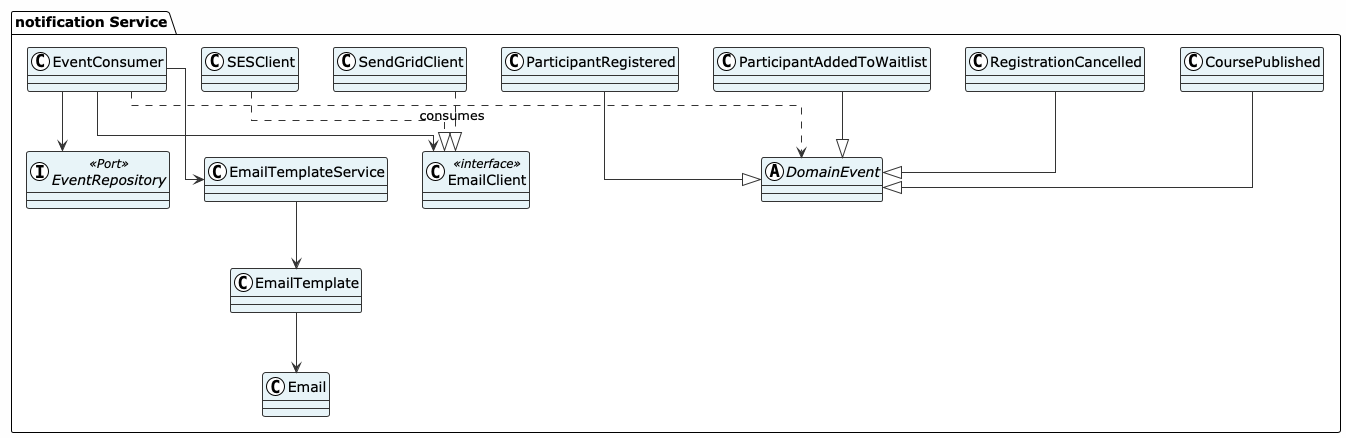
\includegraphics[width=\textwidth]{assets/ebene2_notification_class_diagram}
  \caption{\textit{Ebene~2 -- UML-Klassendiagramm: Interne
  Bausteine des \texttt{notification}-Service.}}
  \label{fig:notification}
\end{figure}

Wichtige Klassen:
\begin{itemize}[leftmargin=1.5em]
  \item \textbf{EventConsumer}: Liest Domain Events aus dem
  Message Broker (RabbitMQ) und delegiert an
  \texttt{EmailTemplateService}.
  \item \textbf{EmailTemplateService}: Wählt das passende
  Template basierend auf Event-Typ und rendert die
  E-Mail mit Event-Daten.
  \item \textbf{TemplateRegistry}: Zentrales Verzeichnis aller
  E-Mail-Templates (z.\,B.\ Bestätigung, Warteliste,
  Stornierung).
  \item \textbf{EmailClient} (Interface): Abstrahiert den
  konkreten E-Mail-Anbieter. Implementierungen:
  \texttt{SESClient} (Amazon SES) oder
  \texttt{SendGridClient} (SendGrid).
  \item \textbf{Email}: Value Object mit Empfänger, Betreff,
  HTML-Body.
\end{itemize}

\noindent\textbf{Domain Events (konsumiert):}
\begin{itemize}[leftmargin=1.5em, label=\raisebox{0.25ex}{\tiny\(\bullet\)}]
  \item \texttt{ParticipantRegistered} -- Bestätigungsmail versenden
  \item \texttt{ParticipantAddedToWaitlist} -- Wartelistenbestätigung versenden
  \item \texttt{RegistrationCancelled} -- Stornierungsbestätigung versenden
  \item \texttt{CoursePublished} -- Ankündigung an Interessenten versenden
\end{itemize}

\paragraph{Event-getriebener Versand}

Der \texttt{notification}-Service ist vollständig
\emph{event-getrieben}: Er hat keine eigene Geschäftslogik,
sondern reagiert nur auf Events, die von anderen Services
publiziert werden. Dies hat mehrere Vorteile:

\begin{itemize}[leftmargin=1.5em]
  \item \textbf{Entkopplung}: Andere Services müssen nicht
  wissen, dass E-Mails versendet werden.
  \item \textbf{Fehlertoleranz}: Sollte der
  \texttt{notification}-Service ausfallen, blockiert
  dies nicht die Einschreibung oder Planung.
  \item \textbf{Skalierbarkeit}: E-Mail-Versand ist
  zeitaufwändig. Durch asynchrone Events kann der
  Service unabhängig skaliert werden.
  \item \textbf{Wartbarkeit}: Template-Änderungen erfordern
  keine Änderungen an anderen Services.
\end{itemize}

% ══════════════════════════════════════════════
\subsection{Ebene~2 -- Bounded Context: \texttt{identity}}
\label{sec:baustein-identity}

Der \texttt{identity}-Service ist ein dünner Adapter zwischen
EduPlanner und dem externen Identity Provider (Keycloak via
OIDC). Er verwaltet keine Passwörter oder Credentials, sondern
delegiert alle Authentifizierung an den IdP und cached nur
Rollen und Berechtigungen. Abbildung~\ref{fig:identity} zeigt
die internen Bausteine und deren Zusammenspiel.

\begin{figure}[H]
  \centering
  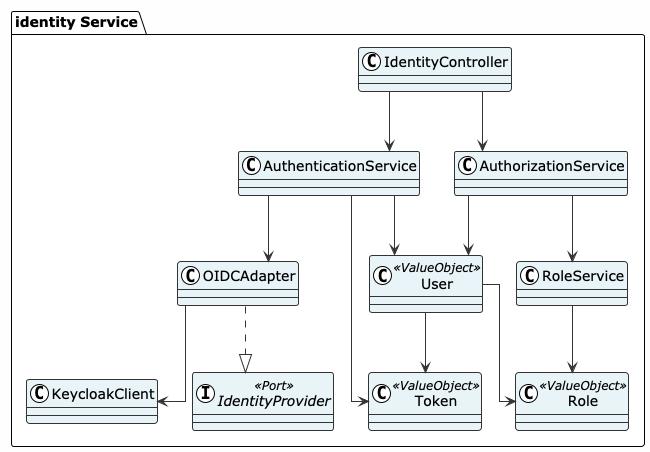
\includegraphics[width=\textwidth]{assets/ebene2_identity_class_diagram}
  \caption{\textit{Ebene~2 -- UML-Klassendiagramm: Interne
  Bausteine des \texttt{identity}-Service.}}
  \label{fig:identity}
\end{figure}

Wichtige Klassen:
\begin{itemize}[leftmargin=1.5em]
  \item \textbf{AuthenticationService}: Orchestriert den
  Authentifizierungsprozess. Delegiert an
  \texttt{OIDCAdapter} und \texttt{TokenValidator}.
  \item \textbf{OIDCAdapter}: Kommuniziert mit dem externen
  Identity Provider (Keycloak). Implementiert das
  OpenID Connect Protokoll.
  \item \textbf{TokenValidator}: Validiert eingehende
  JWT-Tokens auf Signatur, Ablaufdatum und Gültigkeit.
  \item \textbf{AuthorizationService}: Prüft Berechtigungen
  basierend auf Rollen und Permissions.
  \item \textbf{RoleService}: Managed den Cache von
  Benutzerrollen. Wird bei jedem Login aktualisiert.
  \item \textbf{AuthorizationInterceptor}: Wird von anderen
  Services aufgerufen, um Rollen zu prüfen.
\end{itemize}

\paragraph{Authentifizierung vs. Autorisierung}

Der \texttt{identity}-Service trennt zwei kritische Konzepte:

\begin{itemize}[leftmargin=1.5em]
  \item \textbf{Authentifizierung} (``Wer bist du?''):
  Erfolgt via OIDC beim externen IdP (Keycloak).
  Der Service speichert Passwörter \emph{nicht}.
  Stattdessen erhält der Benutzer einen JWT-Token,
  der in allen nachfolgenden Anfragen mitgesendet wird.
  \item \textbf{Autorisierung} (``Darfst du das?''):
  Erfolgt lokal im \texttt{identity}-Service.
  Der Service cached die Rollen des Benutzers
  (z.\,B.\ ``Trainer'', ``Staff'', ``Admin'') und
  prüft, ob diese die angeforderte Aktion erlauben
  (z.\,B.\ ``Darf dieser Benutzer einen Kurs
  löschen?'').
\end{itemize}

\paragraph{Sicherheitsaspekte}

\begin{itemize}[leftmargin=1.5em]
  \item \textbf{Keine Passwörter im System}: Alle
  Authentifizierung erfolgt via Keycloak. EduPlanner
  sieht niemals Passwörter.
  \item \textbf{JWT-Tokens mit Ablaufdatum}: Tokens sind
  zeitlich begrenzt gültig (z.\,B.\ 1~Stunde).
  Nach Ablauf muss der Benutzer sich neu
  authentifizieren.
  \item \textbf{Token-Signatur}: Tokens sind mit einem
  geheimen Schlüssel signiert. Manipulierte Tokens
  werden erkannt.
  \item \textbf{Role-based Access Control (RBAC)}:
  Berechtigungen werden granular auf Rollenebene
  gesteuert. Neue Rollen können im IdP hinzugefügt
  werden, ohne EduPlanner zu ändern.
\end{itemize}

\noindent\textbf{Domain Events:}
\begin{itemize}[leftmargin=1.5em, label=\raisebox{0.25ex}{\tiny\(\bullet\)}]
  \item \texttt{UserCreated} -- Neuer Benutzer wurde angelegt (Admin oder IdP-Sync)
  \item \texttt{UserRoleAssigned} -- Rolle wurde einem Benutzer zugewiesen
\end{itemize}

\begin{hinweis}[Hinweis: Domain Events im \texttt{identity}-Context]
  Diese Events dienen ausschliesslich internen Administrationszwecken
  (z.\,B.\ Audit-Log, Kap.~8.2). Kein anderer Bounded Context konsumiert
  sie im Kernprozess. Sie erscheinen in der vollständigen Event-Übersicht
  (Kap.~12.2 und Anhang~A) der Vollständigkeit halber.
\end{hinweis}
